\documentclass[portrait]{ppgcaposter}
\usepackage{tikz}

\usetikzlibrary{matrix, positioning, decorations.pathreplacing}

\begin{document}

\printheader

\begin{center}
%% TITLE
\textbf{\bf\veryHuge\color{NavyBlue}Estudo do efeito de variações de \textit{Bloom filters} no desempenho de algoritmos de hifenização de palavras\\[1.5cm]}

%% AUTHORS

\huge Matheus Barbosa Silva \\[0.3cm]
\huge Departamento de Ciência da Computação, IME/USP\\[0.3cm]
\Large {\tt{matheus\_barbosa137@usp.br}}

 \end{center}

\vspace{2cm}

%%%% Retire os comentários se houver RESUMO %%%%
%%%%
% \color{Navy}
% \begin{abstract}

%   Te ancillae contentiones vix, ad partiendo patrioque inciderint
%   eum. Mea porro regione ex. Case iuvaret ocurreret quo at, legere
%   malorum indoctum cu his. Eros ubique mel in. At duo partem vidisse
%   intellegam. Equidem detraxit has ea. Phasellus imperdiet, tortor
%   vitae congue bibendum, felis enim sagittis lorem, et volutpat ante
%   orci sagittis mi. Morbi rutrum laoreet semper. Morbi accumsan enim
%   nec tortor consectetur non commodo nisi sollicitudin. Proin
%   sollicitudin. Pellentesque eget orci eros. Fusce ultricies, tellus
%   et pellentesque fringilla, ante massa luctus libero, quis tristique
%   purus urna nec nibh.
  
% \end{abstract}

% \vspace{1cm}

% As FONTES podem ser aumentadas para
% \large \Large \LARGE \huge \Huge \veryHuge \VeryHuge \VERYHuge

 \Large

\begin{multicols}{2} % begin two columns

  \color{black}
  
\section*{Resumo}
A técnica de \textit{cuckoo hashing} é utilizada pelo \textit{cuckoo filter}, estrutura de dados capaz de responder a testes de membresia. Essa é uma estrutura alternativa aos \textit{Bloom filters} que usualmente apresenta melhor desempenho de consultas e menor consumo de espaço em várias aplicações práticas. Tais vantagens são demonstradas em um algoritmo hifenizador de palavras.

\section*{Principais objetivos}

% \color{DarkSlateGray} % DarkSlateGray color for the rest of the content

\begin{enumerate}
\item Descrever o funcionamento de \textit{Bloom filters} e \textit{Cuckoo filters};
\item Comparar o desempenho dessas estruturas em algoritmos de hifenização.
\end{enumerate}

\section{\textit{Bloom filters}}

O \textit{Bloom filter}, estrutura de dados aleatorizada concebida por Bloom \cite{bloom}, tem o objetivo de responder a testes de membresia com \textbf{eficiência no consumo de espaço}. Essa estrutura permite representar os elementos de um conjunto de forma compacta com o custo de resultados \textbf{falsos positivos} -- quando a estrutura responde que um elemento é membro do conjunto, quando de fato não é.

Um \textit{Bloom filter} que representa um dado conjunto $S$ funciona a partir de um vetor booleano de $m$ bits (inicialmente zerado) e $k$ funções de \textit{hashing} universais independentes ($h_1, \dots, h_k$) utilizadas pelo filtro, $h_i: \mathcal{U} \to [0, m-1], \forall i \in [1, k]$. Para a \textbf{inserção} de um dado elemento $x$ na estrutura, todos os bits de índices $h_i(x), \forall i \in [1,k]$ recebem o valor 1. Para verificar se um dado elemento pertence ao conjunto, basta verificar se os $k$ bits indicados pelas funções  de \textit{hashing} contêm o valor 1, caso contrário o resultado é negativo -- tais processos são ilustrados na Figura~1.

\begin{center}\vspace{1cm}
    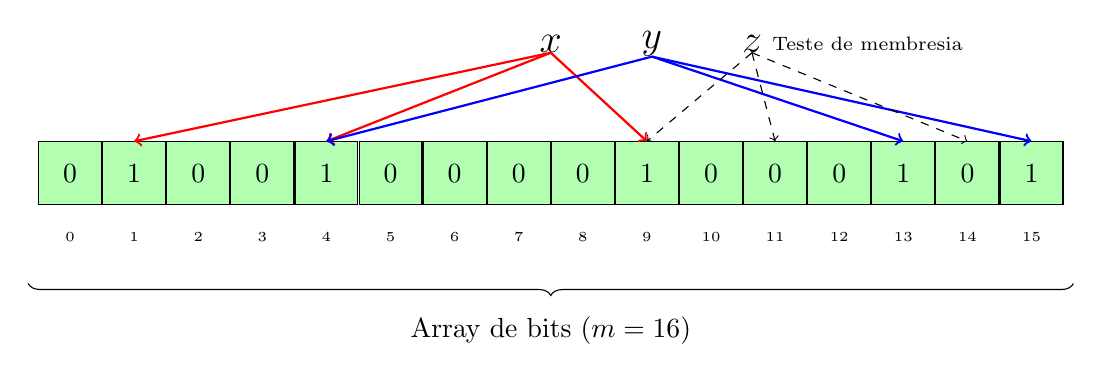
\begin{tikzpicture}[array/.style={matrix of nodes,nodes={anchor=center, draw, minimum size=8mm, fill=green!30},nodes in empty cells, 
    row 2/.style={nodes={font=\tiny,draw=none, fill=none, minimum size=8mm}}}, every label/.append style={font=\scriptsize}]

            \matrix[array] (array) {
        
          0 & 1 & 0 & 0 & 1 & 0 & 0 & 0 & 0 & 1 & 0 & 0 & 0 & 1 & 0 & 1\\
          0 & 1 & 2 & 3 & 4 & 5 & 6 & 7 & 8 & 9 & 10 & 11 & 12 & 13 & 14 & 15\\};
          \node[above=of array, font=\Large, inner sep=0] (x) {$x$};
          \node[right=of x, font=\Large, inner sep=0] (y) {$y$};
          \node[right=of y, font=\Large, inner sep=0, label={right:Teste de membresia}] (z) {$z$};0
          
          \draw[thick,->,draw=red] (x.south) -- (array-1-2.north) node[above, pos=0.8] {};
          \draw[thick,->,draw=red] (x.south) -- (array-1-5.north) node[above, pos=0.8] {};
          \draw[thick,->,draw=red] (x.south) -- (array-1-10.north) node[above, pos=0.8] {};

          \draw[thick,->,draw=blue] (y.south) -- (array-1-5.north) node[above, pos=0.8] {};
          \draw[thick,->,draw=blue] (y.south) -- (array-1-14.north) node[above, pos=0.8] {};
          \draw[thick,->,draw=blue] (y.south) -- (array-1-16.north) node[above, pos=0.8] {};

          \draw[dashed,->] (z.south) -- (array-1-10.north) node[above, pos=0.8] {};
          \draw[dashed,->] (z.south) -- (array-1-12.north) node[above, pos=0.8] {};
          \draw[dashed,->] (z.south) -- (array-1-15.north) node[above, pos=0.8] {};
          \draw[decorate, decoration={brace, amplitude=1ex, raise=1cm}] (array.east) -- node[midway, below=1.3cm] {Array de bits ($m=16$)} (array.west);
        \end{tikzpicture}
\captionof{figure}{ Esquema do funcionamento de um \textit{Bloom filter} com parâmetros $m=16, k=3, n=2, S = \{x, y\}$ com teste de membresia do elemento $z$ que não pertence à estrutura}
\end{center}\vspace{1cm}

\section{\textit{Cuckoo filters}}

O \textit{cuckoo filter}, descrito por Fan \textit{et al.} \cite{cuckoo}, é proposto como uma alternativa ao \textit{Bloom filter} tradicional para os cenários em que a \textbf{remoção de elementos} da estrutura é necessária. Para isso, utiliza-se o \textbf{\textit{cuckoo hashing}} como um modo de construção do filtro. Essa estrutura é composta por um vetor de \textit{buckets} e duas funções de \textit{hashing} $h_1(x)$ e $h_2(x)$ que mapeiam um dado elemento $x$ para dois \textit{buckets} da estrutura.

Para a inserção, caso algum dos dois \textit{buckets} de índices dados pelas funções de \textit{hashing} tenha espaço para um novo elemento, $x$ é inserido no \textit{bucket} disponível. Caso contrário, seleciona-se um dos dois \textit{buckets} e $x$ toma o lugar de um elemento anteriormente inserido. Nesse cenário, o elemento removido é \textbf{realocado} (esse processo é ilustrado na Figura~2).

Essa estrutura é especialmente vantajosa com relação aos Bloom filters tradicionais pois permite que elementos sejam removidos da estrutura dinamicamente, tem melhor desempenho em consultas e usualmente consome menos espaço se a razão de falsos positivos $\epsilon$ alvo é menor que 3\%.

\begin{center}\vspace{1cm}
    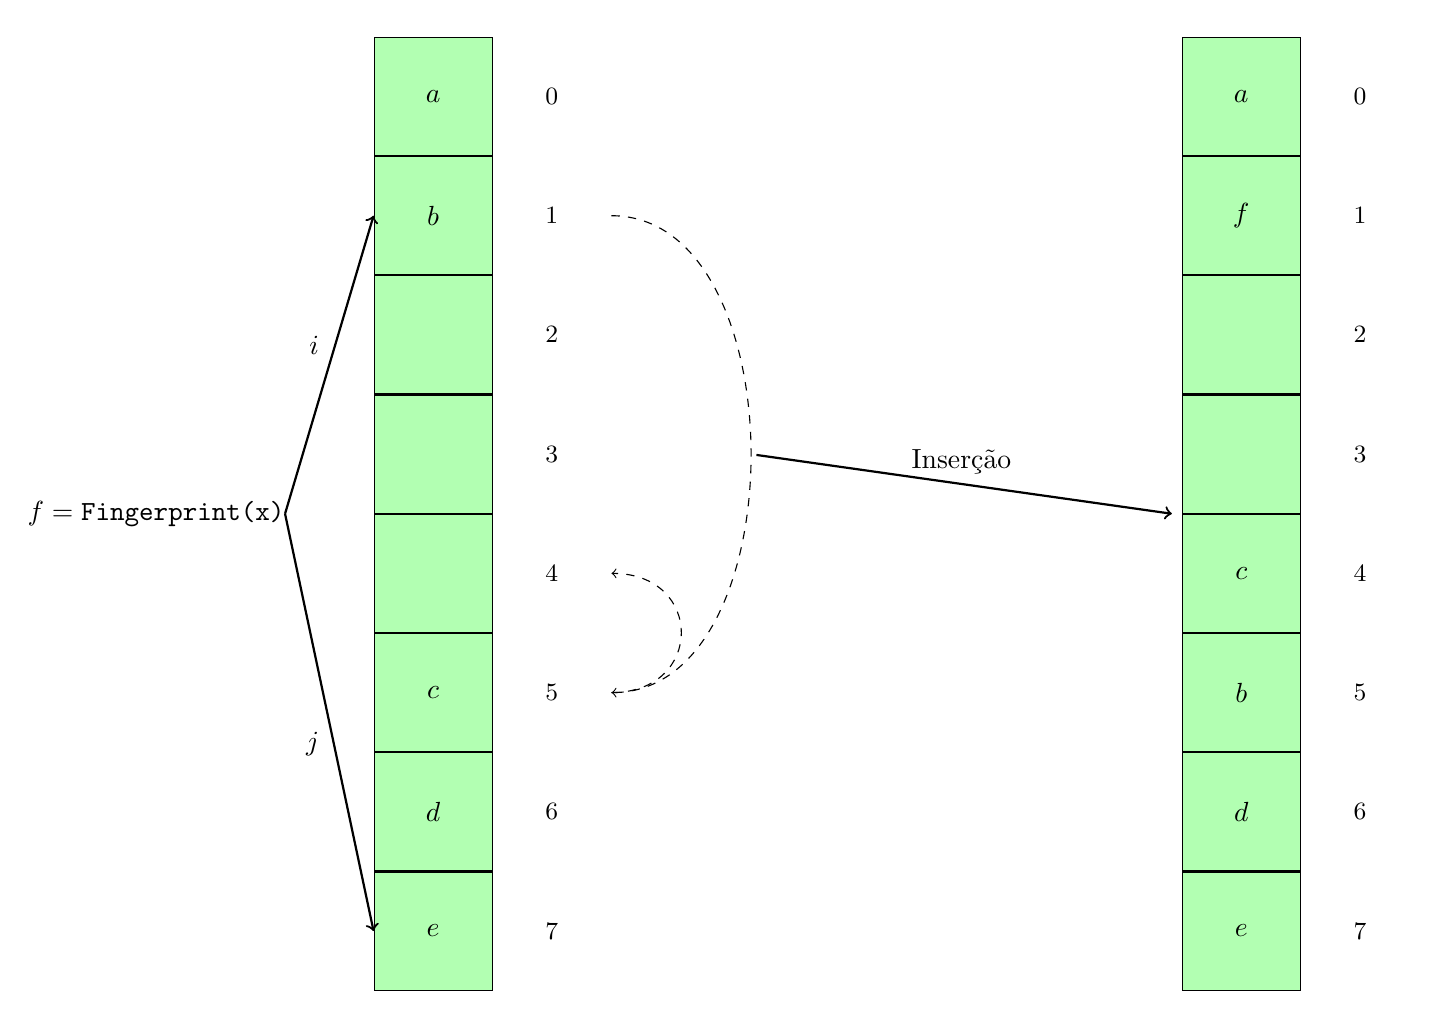
\begin{tikzpicture}[array/.style={matrix of nodes,nodes={anchor=center, draw, minimum size=15mm, fill=green!30}, nodes in empty cells, 
column 2/.style={nodes={font=\small,draw=none, fill=none, minimum size=15mm}}}]

            \matrix[array] (array) {
               $a$ & 0\\
               $b$ & 1\\
                & 2\\
                & 3\\
                & 4\\
                $c$ & 5\\
                $d$ & 6\\
                $e$ & 7\\
            };
          \node[left=of array, inner sep=0] (f) {$f = \texttt{Fingerprint(x)}$};
          
          \draw[thick,->] (f.east) -- (array-2-1.west) node[midway, above left] {$i$};
          \draw[thick,->] (f.east) -- (array-8-1.west) node[midway, below left] {$j$};

          \draw[dashed,->] (array-6-2.east) to [out=0,in=0, looseness=2] (array-5-2.east);
          \draw[dashed,->] (array-2-2.east) to [out=0,in=0, looseness=1] coordinate[pos=0.5] (seta) (array-6-2.east);

          \matrix[right=of array, shift={(6cm,0)}, array] (arrayInsert) {
               $a$ & 0\\
               $f$ & 1\\
                & 2\\
                & 3\\
                $c$ & 4\\
                $b$ & 5\\
                $d$ & 6\\
                $e$ & 7\\
            };
            \draw[thick,shorten <=2pt, ->] (seta.east) -- (arrayInsert.west) node[midway, above] {Inserção};
        \end{tikzpicture}
\captionof{figure}{Esquema do funcionamento da inserção de um elemento $x$ em um \textit{Cuckoo filter} com a técnica de \textit{partial-key cuckoo hashing}}
\end{center}\vspace{1cm}

\section{Experimentos}

De acordo com Bloom \cite{bloom}, a aplicação de \textit{Bloom filters} é vantajosa em algoritmos hifenizadores de palavras. Modifica-se o algoritmo \texttt{hypher}, um hifenizador de palavras popular, de modo a criar duas versões: uma que utiliza \textit{Bloom filters} e outra que utiliza \textit{Cuckoo filters}. O tempo médio de cada versão para hifenizar um mesmo dicionário é exibido na Figura~3.

Nota-se que as estruturas apresentam, nos experimentos realizados, tempos médios de hifenização relativamente próximos, ainda que a versão com \textit{cuckoo filter} consuma menos espaço.


\begin{center}\vspace{1cm}
    \includegraphics[width=0.9\linewidth]{cuckoo-bloom-comparison.png}
    \captionof{figure}{Comparação entre os tempos médios de execução de um mesmo algoritmo hifenizador de palavras implementado com \textit{Bloom filter} e com \textit{cuckoo filter}}
\end{center}\vspace{1cm}

\section{Conclusões}

\begin{itemize}
\item \textit{Cuckoo filters} podem substituir \textit{Bloom filters} em algoritmos hifenizadores de palavras, de modo que o consumo de tempo se mantenha similar para qualquer $\epsilon$, mas com menor consumo de espaço;
\item O tempo de construção dessas estruturas é, também, semelhante.
\end{itemize}

\bibliographystyle{plain} % Plain referencing style
\bibliography{refs} % Use the example bibliography file %sample.bib

\end{multicols}

\end{document}